\documentclass[11pt, oneside]{article}   	% use "amsart" instead of "article" for AMSLaTeX format
\usepackage{geometry}                		% See geometry.pdf to learn the layout options. There are lots.
\geometry{letterpaper}                   		% ... or a4paper or a5paper or ... 
%\geometry{landscape}                		% Activate for rotated page geometry
%\usepackage[parfill]{parskip}    		% Activate to begin paragraphs with an empty line rather than an indent
\usepackage{graphicx}				% Use pdf, png, jpg, or eps§ with pdflatex; use eps in DVI mode
								% TeX will automatically convert eps --> pdf in pdflatex		
\usepackage{amssymb}

%SetFonts

%SetFonts


\title{Prediction of Septic Shock for ICU patients with chronic diseases}
\author{Ya Ting Chang, Michelle Hsu}
%\date{}							% Activate to display a given date or no date

\begin{document}
\maketitle
\section{Experimental Setup}
\subsection{Cohort Selection}
The dataset used in this study is the from MIMIC II (Multiparameter Intelligent Monitoring in Intensive Care), which is the clinical data collected from Beth Israel Deaconess Medical�Center.
Since our study focuses on patients with chronic diseases, the cohort is comprised of ICU patients with diabetes, chronic kidney diseases, and chronic lung diseases.

\begin{table}[htbp]
  \centering 
  \begin{tabular}{|p{4cm}|p{2cm}|p{2cm}|p{2cm}|}
  \hline 
    & Diabetes(\%) & Kidney(\%) & Lung(\%)\\ 
    \hline \\[-11pt]
    Sepsis (n=40) & 80 &  25 & 15 \\ 
    Severe Sepsis (n=217) & 73.3 &  29.9 & 10.1\\
    Septic Shock (n=109) & 72.5 & 24.8 & 11.9\\
     \hline 
  \end{tabular}
  \label{tab:example} 
    \caption{Chronic Disease(\%) for each Syndrome} 
\end{table}

\begin{table}[htbp]
  \centering 
  \begin{tabular}{lclc} 
    & Mean & Median \\ 
    \hline \\[-11pt]
    Blood Pressure & 76.01 & 74.87 \\ 
    Heart Rate & 85.18 & 84.02\\
    Respiratory Rate & 19.98 & 19.52\\
    Oxygen Saturation & 96.75 & 97.24\\
    Temperature & 98.05 & 98.10\\
     \hline 
  \end{tabular}
  \label{tab:example} 
    \caption{Vital Signs Statistics of Chronic Disease Patients (n=1,640)} 
\end{table}

\subsection{Data Extraction}
Extracted from the MIMIC II dataset, we utilized the tables containing hospitalization information, vital signs measurement, patient demographics, and medical diagnosis. Regarding the data preprocessing, we first identify the code of our interested chronic diseases (diabetes, kidney, and lung) and the targets (sepsis, severe sepsis, and septic shock). We then filter the hospitalization (hadm\_id) with the identified chronic disease. For these selected hospitalizations, we used one-hot encoding to transform the three diseases into the binary representation. As for the outcome variables, we also conducted the binary transformation and joined the two wide-format tables using column ?hadm\_id?, resulting in a table with each row representing a unique hospitalization. For the next step, we added other features such as the vital signs and demographic information to the wide-format table by hadm\_id. In the original data from MIMIC II, each instance represents a unique ICU stay. Therefore, one hospitalization can have several records of the same vital sign since a patient can be admitted to ICU more than one time per hospitalization. To address the multiple records issue, we averaged the vital sign measurements among the ICU stays to represent the unique hospitalization. After the data preprocessing, the final table contains 1,640 rows with 20 features. For our analysis, we assumed each hospitalization is independent and treated each hospitalization as one instance.

Before running the model, we handled the problems of missing values and imbalanced data in our dataset. Regarding the missing values, the issue primarily comes from the vital sign features with blood pressure containing the highest percentage (7.99\%) of missing values. We adopted MICE (Multivariate Imputation by Chained Equations) as our imputation method with the assumption that the values are missing at random. As for the imbalanced data, we implemented SMOTE (Synthetic Minority Over-Sampling Technique) to overcome the skewed dataset. SMOTE incorporates the k nearest neighbor as the underlying method to over-sample the minority class and under-sample the majority class. 

\begin{table}[htbp]
  \centering 
  \begin{tabular}{lclc}
  \hline 
    & Missing Value(\%) \\ 
    \hline \\[-11pt]
    Sex & 0.366\\ 
    Age & 0.122\\
    Blood Pressure & 7.99\\
    Heart Rate & 4.82\\
    Respiratory Rate & 5.06\\
    Oxygen Rate & 5.06\\
    Temperature & 6.52\\
     \hline 
  \end{tabular}
  \label{tab:example} 
    \caption{Missing value(\%) of predictors} 
\end{table}

\begin{table}[htbp]
  \centering 
  \begin{tabular}{|p{3cm}|p{3cm}|p{3cm}|p{3cm}|}
  \hline 
    & Sepsis(\%) & Severe Sepsis(\%) & Septic Shock(\%)\\ 
    \hline \\[-11pt]
    Original & 2.44 &  13.2 & 6.65 \\ 
    SMOTE & 26.8 &  42.9 & 27.6\\
     \hline 
  \end{tabular}
  \label{tab:example} 
    \caption{Imbalanced data(\%) with SMOTE} 
\end{table}

\subsection{Feature Choices}
The features in this study is composed of 4 categories?demographics, vital signs, chronic disease indicator, and the outcome variables. The original variables including race and diagnosis were converted to dummy variables with the binary representation since we want to assess the importance of each variable in terms of the 3 syndromes. To implement random forest and gradient boosting algorithms, we then transformed the outcome variables (sepsis, severe sepsis, and septic shock) into categorical variables. 
 
\begin{table}[htbp]
  \centering 
  \begin{tabular}{|p{2.7cm}|p{13cm}|}
  \hline 
    & Feature\\ 
    \hline \\[-11pt]
    Demographic &  age, sex, white, asian, black, hispanic, others, unknown\\ 
    Vital Signs & blood.pressure, heart.rate, respiratory.rate, oxygen.saturation, temperature\\
    Chronic Disease & diabetes, kidney, lung\\
    Outcome & Sepsis, SeverSepsis, SepticShock\\
     \hline 
  \end{tabular}
  \label{tab:example} 
    \caption{Feature Selection} 
\end{table}

\subsection{Comparison Methods}
Our analysis used the similar approach with the study from BMJ Journal, which implemented ensemble machine learning techniques to evaluated the existing sepsis prediction algorithm (InSight). Compared to the study which adopted 10-fold cross validation on gradient boosting method to predict the onset of sepsis, severe sepsis, and septic shock, we used only 5-fold cross validation yet incorporated the tuning process on the max depth of each tree and the number of boosting iterations. 
\subsection{Evaluation Criteria}
Besides the accuracy rate, we assessed our models with ROC curve and AUC to ensure the result is not biased by the skewness of the dataset even though we handled the imbalanced data using SMOTE in the earlier step. 

\begin{figure}[htbp]
  \centering 
  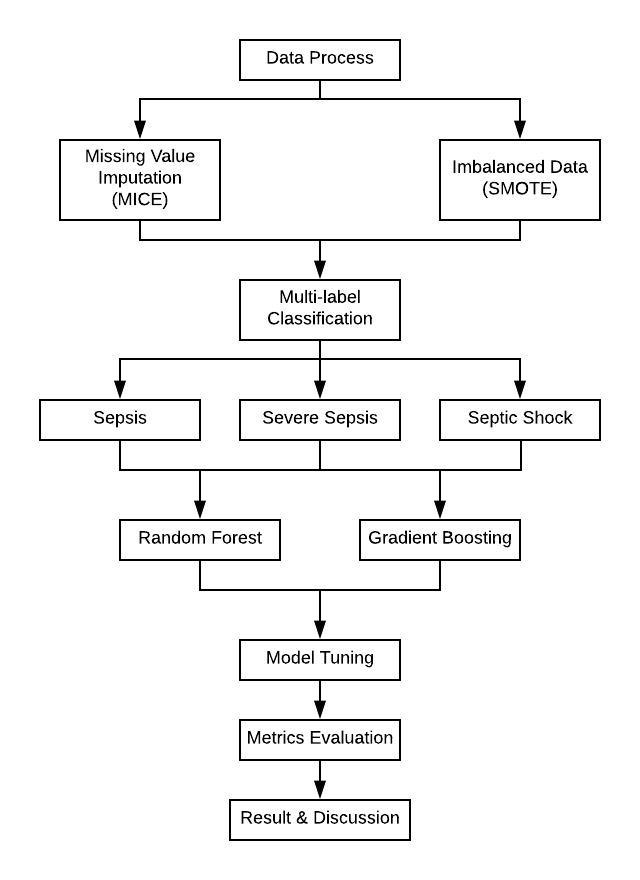
\includegraphics[width=2.5in]{Pipeline.jpeg} 
  \caption{Pipeline}
  \label{fig:example} 
\end{figure} 

\section{Discussion and Related Work }
Based on the result of our study, we can conclude that vital signs are important indicators for predicting the onset of sepsis, severe sepsis, and septic shock, which is in line with the findings from the paper by BMJ Journal. Also, for different levels of sepsis condition, certain race exhibits different level of importance for the prediction. For instance, race black is an important variable while predicting septic shock. Therefore, by taking race into consideration, doctors can be more informed of the risk of sepsis condition for the patients with chronic diseases. However, there are some limitations for the study. We only focused on the ICU patients with certain type of chronic diseases (diabetes, kidney diseases, and lung disease). Hence, the result only applies to patients with the specific medical condition. The other limitation is derived from the small sample size of the analysis. Our models were constructed upon 1,640 instances, which may generate different results with larger sample size. In addition, MIMIC II is not the most updated dataset. The clinical data only ranges from 2001 to 2008. To generalize our study, we will need to use a more recent dataset from MIMIC III.

\section{Conclusion}
In sum, the study focuses on the prediction of the onset of sepsis-related condition for ICU patients with diabetes, chronic kidney disease, or chronic lung disease. We divided the original multi-label classification problem into 3 binary classification tasks and leveraged the ensemble machine learning method with Na�ve Bayes as our baseline. For future extension on the study, we will include other types of chronic diseases such as cancer and cardiovascular disease. Additionally, using a more up-to-date database such as MIMIC III to analyze sepsis-related syndromes will also be our focus.

\end{document}  